% Indicate the main file. Must go at the beginning of the file.
% !TEX root = ../main.tex

%----------------------------------------------------------------------------------------
% CHAPTER TEMPLATE
%----------------------------------------------------------------------------------------


\chapter{Resultate} % Main chapter title

\label{Chapter4} % Change X to a consecutive number; for referencing this chapter elsewhere, use \ref{ChapterX}

%----------------------------------------------------------------------------------------
% SECTION 1
%----------------------------------------------------------------------------------------
In diesem Kapitel werden die Ergebnisse der verschiedenen Analysen erläutert.
\section{Ergebnisse Racetrack}
Erste Analysen zeigen....
\section{Ergebnisse Latency vs. Churn}
Die verschiedenen Farben in der  \autoref{fig:pr-latency-vs-churn-allgemein}  repräsentieren die einzelnen Projekte der Projektgruppen.
Wie in der Abbildung ersichtlich, zeigt sich ein Cluster von Datenpunkten in der linken unteren Ecke. Dabei konzentrieren sich die Punkte vorallem bei einem Churn von unter 1000 Zeilen und unter 100 Stunden Latency. Es wird deutlich, dass sowohl hohe Churn-Werte schnell abgearbeitet werden, wie auch niedrige Churn-Werte hohe Latencies aufweisen. Die vorliegende Grafik gibt keinerlei Tendenzen zu einer Korrelation zwischen den Metriken Latency und Churn wieder.
\begin{figure}[th]
    \centering
    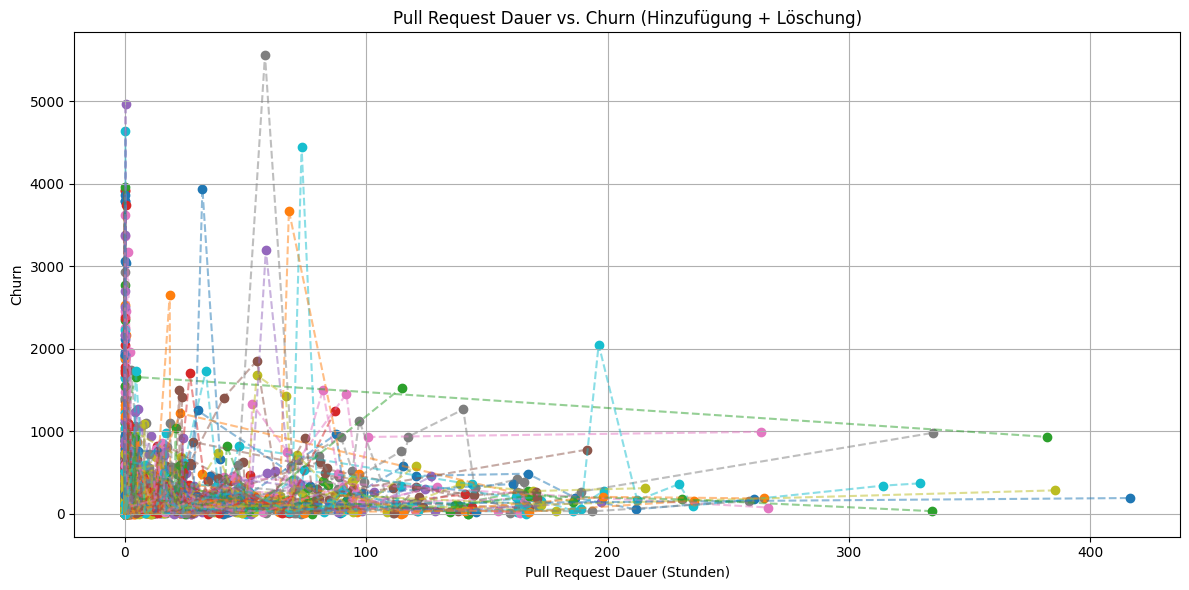
\includegraphics[width=\textwidth]{pr-latency-vs-churn-allgemein.png}
    \caption{Scatterplot der Churn-Werte in Relation zur PR-Latenz}
    \label{fig:pr-latency-vs-churn-allgemein}
\end{figure}

Dies wird ebenfalls durch die Berechnung des Spearman Rangkorrelationskoeffizienten deutlich, der bei einem Wert von 0,17 keine monotone Korrelation aufzeigt.

// TODO übergang

Die Auswertung der Daten ergibt, dass die Latency in den Vollzeitklassen mit 0.8 Stunden nahezu doppelt so hoch ist wie in den Teilzeitklassen, wo der Mittelwert bei 0.46 liegt. Bei den Churn-Werten ist hingegen kein signifikanter Unterschied erkennbar. Dies ist in der nachfolgenden \autoref{fig:vergleich-latency-churn} ersichtlich.

\begin{figure}[ht]
    \centering
    \begin{subfigure}[b]{0.48\textwidth}
        \centering
        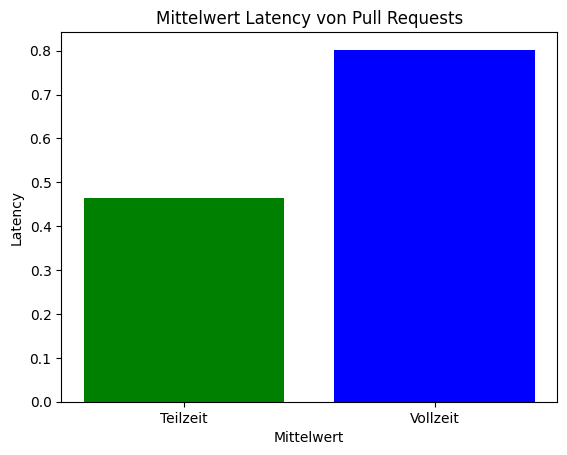
\includegraphics[width=\textwidth]{Figures/mittelwert-latency-t-v.png}
        \caption{Mittelwerte Latency Vollzeit vs. Teilzeit}
        \label{fig:mittelwert-latency-t-v}
    \end{subfigure}
    \hfill
    \begin{subfigure}[b]{0.48\textwidth}
        \centering
        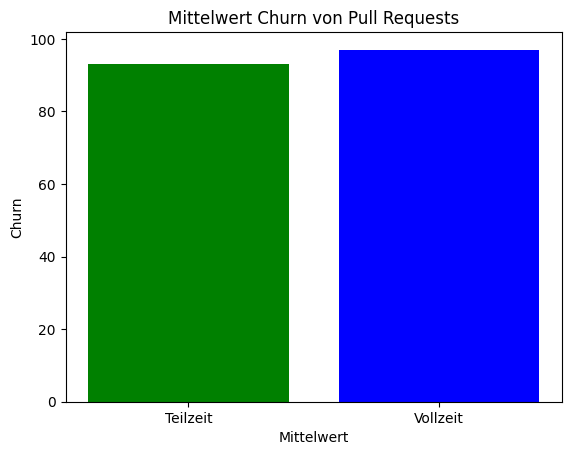
\includegraphics[width=\textwidth]{Figures/mittelwert-churn-t-v.png}
        \caption{Mittelwerte Churn Vollzeit vs. Teilzeit}
        \label{fig:mittelwert-churn-t-v}
    \end{subfigure}
    \caption{Vergleich von Latency und Churn zwischen Vollzeit und Teilzeit}
    \label{fig:vergleich-latency-churn}
\end{figure}

Eine detaillierte Analyse der Latencies von Teilzeit- und Vollzeitstudierenden offenbart, dass Teilzeitklassen eine signifikant höhere Anzahl an Pull Requests aufweisen, die innerhalb einer Minute abgeschlossen werden. Dies zeigt sich im ersten Säulenpaar bei der \autoref{fig:anz-prs-vs-latency-tv}. Der Anteil der innerhalb einer Minute abgeschlossenen Pull Requests beläuft sich auf 16.8 Prozent der Gesamtzahl der Pull Requests bei den Teilzeitstudierenden, während dieser Anteil bei den Vollzeitstudierenden 9.9 Prozent beträgt. Bei allen Zeitabschnitten ausser 4–8 Stunden und 8–12 Stunden zeigen die Teilzeitklassen eine grössere Anzahl an Pull Requests, jedoch sind die grössten Differenzen bei den ersten drei und dem letzten Säulenpaar erkennbar. Eine Zusammenfassung der Pull Requests von 0 bis 30 Minuten ergibt, dass diese bei den Teilzeitklassen 50.7 Prozent und bei den Vollzeitklassen 44.7 Prozent ausmachen. Die letzte Säule zeigt einen Anteil von 18.6 Prozent für Teilzeitklassen und 19.7 Prozent für Vollzeitklassen. 
\begin{figure}[htbp]
    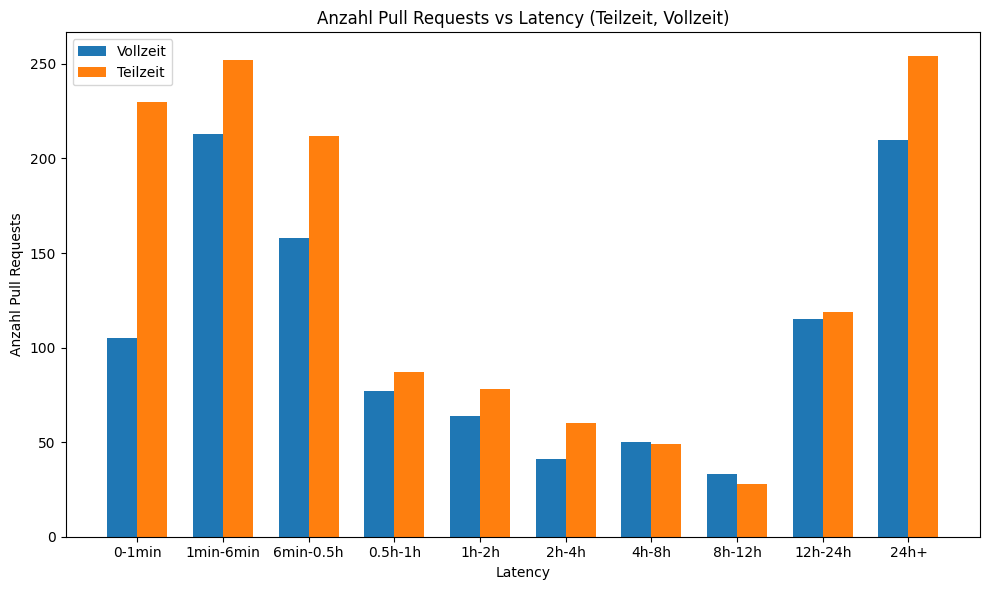
\includegraphics[width=\textwidth]{Figures/anz-prs-vs-latency-tv.png}
    \caption{Anzahl PullRequests vs. Latency (Teilzeit, Vollzeit)}
    \label{fig:anz-prs-vs-latency-tv}
\end{figure}

// TODO keine dev branches?
\newpage
\subsection{Ergebnisse Einfluss Projektzeit}
\begin{figure}[htbp]
    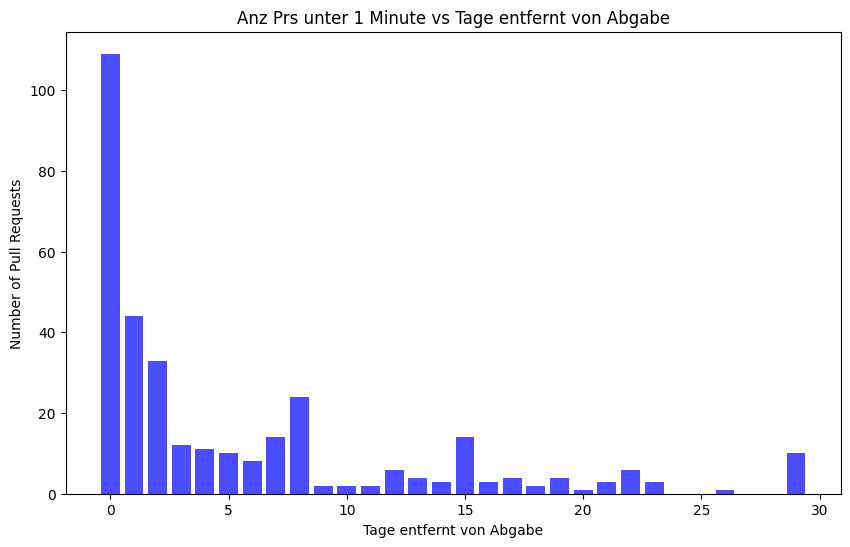
\includegraphics[width=\textwidth]{Figures/anz-prs-under-1-min.png}
    \caption{Anzahl PullRequests unter einer Minute}
    \label{fig:anz-prs-under-1-min}
\end{figure}
